\documentclass[oneside]{book}

\usepackage{amsmath}
\usepackage{amssymb}
\usepackage{amsthm}
\usepackage{epigraph}
\usepackage{listings}
\usepackage[svgnames]{xcolor}
\usepackage{xcolor}
\usepackage{tikz}
\usepackage{caption}
\usepackage[bookmarks=false, unicode]{hyperref}
\usepackage{float}
\usetikzlibrary{calc, decorations.pathreplacing}
\usepackage{parskip}
\usepackage{booktabs}
\usepackage{geometry}
\geometry{margin=1in}
\usepackage[skins, listings, most]{tcolorbox}
\usepackage{xparse}

\definecolor{backcolour}{rgb}{1,1,1}
\definecolor{codegray}{rgb}{1,1,1}
\definecolor{codeframe}{rgb}{0.35,0.35,0.35}

\newtcblisting{pythoncode}[2][]{
    colback=codegray,
    colframe=codeframe,
    listing only,
    arc=0pt, outer arc=0pt,
    boxrule=0.5pt,
    listing options={
        language=Python,
        basicstyle=\ttfamily\small,
        keywordstyle=\color{blue!80!black}\bfseries,
        commentstyle=\color{green!40!black}\bfseries,
        stringstyle=\color{red!60!black},
        numbers=left,
        numberstyle=\tiny\color{gray},
        stepnumber=1,
        showstringspaces=false,
        tabsize=4,
        breaklines=true
    },
    title=\textbf{Python Code:} #2,
    #1
}

\lstdefinestyle{mystyle}{
    backgroundcolor=\color{backcolour},   
    commentstyle=\color{codegreen},
    keywordstyle=\color{magenta},
    numberstyle=\tiny\color{codegray},
    stringstyle=\color{codepurple},
    basicstyle=\ttfamily\footnotesize,
    breakatwhitespace=false,         
    breaklines=true,                 
    captionpos=b,           
    keepspaces=true,                 
    numbers=left,                    
    numbersep=5pt,                  
    showspaces=false,                
    showstringspaces=false,
    showtabs=false,                  
    tabsize=4
}
\lstset{style=mystyle}

\allowdisplaybreaks
\DeclareMathOperator{\arcsec}{arcsec}
\DeclareMathOperator{\arccot}{arccot}
\DeclareMathOperator{\arccsc}{arccsc}
\DeclareMathOperator{\sech}{sech}
\DeclareMathOperator{\csch}{csch}
\DeclareMathOperator{\arcsinh}{arcsinh}
\DeclareMathOperator{\arccosh}{arccosh}
\DeclareMathOperator{\arctanh}{arctanh}

\newcommand{\preface}{
  \cleardoublepage
  \chapter*{Preface}
  \addcontentsline{toc}{chapter}{Preface}
}

\newtcbtheorem[number within=section]{mydef}{Definition}{
    enhanced,
    breakable,
    colback=blue!5!white,
    colframe=blue!75!black,
    attach boxed title to top left={yshift*=-\tcboxedtitleheight/2},
    fonttitle=\bfseries,
    boxed title style={colback=blue!75!black, colframe=blue!75!black}
}{def}

\newtcbtheorem[number within=section]{mythm}{Theorem}{
    enhanced,
    breakable,
    colback=red!5!white,
    colframe=red!75!black,
    attach boxed title to top left={yshift*=-\tcboxedtitleheight/2},
    fonttitle=\bfseries,
    boxed title style={colback=red!75!black, colframe=red!75!black}
}{thm}

\newtcbtheorem[number within=section]{myproposition}{Proposition}{
    enhanced,
    breakable,
    colback=orange!5!white,
    colframe=orange!80!black,
    attach boxed title to top left={yshift*=-\tcboxedtitleheight/2},
    fonttitle=\bfseries,
    boxed title style={colback=orange!80!black, colframe=orange!80!black}
}{prp}

\newtcbtheorem[number within=section]{myprop}{Property}{
    enhanced,
    breakable,
    colback=green!5!white,
    colframe=green!60!black,
    attach boxed title to top left={yshift*=-\tcboxedtitleheight/2},
    fonttitle=\bfseries,
    boxed title style={colback=green!60!black, colframe=green!60!black}
}{prop}

\newtcbtheorem[number within=section]{mycor}{Corollary}{
    enhanced,
    breakable,
    colback=violet!5!white,
    colframe=violet!75!black,
    attach boxed title to top left={yshift*=-\tcboxedtitleheight/2},
    fonttitle=\bfseries,
    boxed title style={colback=violet!75!black, colframe=violet!75!black}
}{cor}

\newtcbtheorem[number within=section]{myex}{Example}{
    enhanced,
    breakable,
    colback=teal!5!white,
    colframe=teal!75!black,
    attach boxed title to top left={yshift*=-\tcboxedtitleheight/2},
    fonttitle=\bfseries,
    boxed title style={colback=teal!75!black, colframe=teal!75!black}
}{ex}

\newtcbtheorem[number within=section]{myrem}{Remark}{
    enhanced,
    breakable,
    colback=gray!5!white,
    colframe=gray!75!black,
    attach boxed title to top left={yshift*=-\tcboxedtitleheight/2},
    fonttitle=\bfseries,
    boxed title style={colback=gray!75!black, colframe=gray!75!black}
}{rem}

\newtcolorbox{mynote}{
    enhanced,
    breakable,
    colback=yellow!10!white,
    colframe=orange!85!black,
    title={\textbf{Note}},
    coltitle=black,
    attach boxed title to top left={yshift*=-\tcboxedtitleheight/2},
    boxed title style={colback=orange!50!yellow, colframe=orange!85!black},
    sharp corners=south,
}

\ProvideDocumentEnvironment{definition}{o}
  {\IfValueTF{#1}{\begin{mydef}{#1}{}}{\begin{mydef}{}{}}}
  {\end{mydef}}

\ProvideDocumentEnvironment{theorem}{o}
  {\IfValueTF{#1}{\begin{mythm}{#1}{}}{\begin{mythm}{}{}}}
  {\end{mythm}}

\ProvideDocumentEnvironment{proposition}{o}
  {\IfValueTF{#1}{\begin{myproposition}{#1}{}}{\begin{myproposition}{}{}}}
  {\end{myproposition}}

\ProvideDocumentEnvironment{property}{o}
  {\IfValueTF{#1}{\begin{myprop}{#1}{}}{\begin{myprop}{}{}}}
  {\end{myprop}}

\ProvideDocumentEnvironment{corollary}{o}
  {\IfValueTF{#1}{\begin{mycor}{#1}{}}{\begin{mycor}{}{}}}
  {\end{mycor}}

\ProvideDocumentEnvironment{inference}{o}
  {\IfValueTF{#1}{\begin{mycor}{#1}{}}{\begin{mycor}{}{}}}
  {\end{mycor}}

\ProvideDocumentEnvironment{example}{o}
  {\IfValueTF{#1}{\begin{myex}{#1}{}}{\begin{myex}{}{}}}
  {\end{myex}}

\ProvideDocumentEnvironment{remark}{o}
  {\IfValueTF{#1}{\begin{myrem}{#1}{}}{\begin{myrem}{}{}}}
  {\end{myrem}}

\ProvideDocumentEnvironment{note}{}{\begin{mynote}}{\end{mynote}}

\ProvideDocumentEnvironment{lemma}{o}
  {\IfValueTF{#1}{\begin{mythm}{#1}{}}{\begin{mythm}{}{}}}
  {\end{mythm}}

\begin{document}

\begin{titlepage}

    \definecolor{elegantblue}{RGB}{0, 51, 102}

    \vspace*{3cm}
    {\color{elegantblue}\hrule height 3pt}
    \vspace{1cm}

    \noindent
    {\Huge \bfseries \color{elegantblue} Introduction to Artificial Intelligence\par}

    \vspace{1cm}
    {\color{elegantblue}\hrule height 3pt}

    \vfill
    \begin{flushleft}
        {\Large \textbf{Jinshuo Li}}\\[15pt]
        {\large Shanghai Jiao Tong University}\\[8pt]
        {\large \today}
    \end{flushleft}
    \vspace{2cm}
\end{titlepage}
\thispagestyle{empty}


\cleardoublepage

\pagenumbering{gobble}
\tableofcontents
\thispagestyle{empty}

\cleardoublepage

\preface
\thispagestyle{empty}

Standing at the beginning of 2026, looking back at the tumultuous development of Artificial Intelligence over the past few years, one cannot help but feel a sense of awe. From the initial explosion of generative models to the ubiquity of intelligent agents today, AI has fundamentally reshaped the way we research, work, and live.

However, amidst the dazzling array of applications and the rapid iteration of tools, the underlying principles often remain obscured by the hype. As a student at Shanghai Jiao Tong University, I have spent much of my time navigating through this fog, attempting to connect the classical theories of machine learning with the emergent behaviors of modern large models.

This document is not merely a collection of technical notes; it is an attempt to construct a coherent narrative of AI knowledge as I understand it. It begins with the fundamental mathematics and algorithms, traverses through the architectures that defined the deep learning era, and arrives at the frontier of current research.

My hope is that this work will serve as a roadmap for those who, like me, are eager to look beyond the "black box" and understand the elegant logic that drives the intelligence of our time.

Writing is a process of learning. All errors and omissions are my own, and I welcome any corrections.

\begin{flushright}
Jinshuo Li \\
Shanghai Jiao Tong University \\
2026.1.6, in Beijing
\end{flushright}

\cleardoublepage
\pagenumbering{arabic}
\setcounter{page}{1}
\chapter{Basics}

This is the first chapter of the document. Here we will cover the basic concepts and foundational information necessary for understanding the subsequent chapters.

\section{Language and Packages}

To follow the trends in research of artificial intelligence, we will use \textbf{Python} as the programming language throughout this book. Python is widely adopted in the AI community due to its simplicity and the vast array of libraries available for machine learning, data analysis, and scientific computing.

To be specific, I would like to inform the readers that we use \textbf{3.11.9} version of Python in this book at the time of \today. You can download it from the official Python website: \url{https://www.python.org/downloads/release/python-3119/}. This version is stable and includes the latest features and improvements, while maintaining compatibility with most libraries used in AI research.

Also, we will use several popular Python libraries throughout the book, including but not limited to:

\begin{itemize}
    \item \textbf{NumPy}: For numerical computations and array manipulations.
    \item \textbf{Pandas}: For data manipulation and analysis.
    \item \textbf{Matplotlib} and \textbf{Seaborn}: For data visualization.
    \item \textbf{Pytorch} and \textbf{TensorFlow}: For building and training machine learning models.
\end{itemize}

We have to say that this should be a continuously updating list as new libraries and tools are developed in the fast-evolving field of AI. I encourage readers to stay updated with the latest developments and consider exploring additional libraries that may be relevant to their specific interests and projects.

\newpage

\section{Introduction to Tensor}

A \textbf{tensor} is a mathematical object that generalizes the concepts of scalars, vectors, and matrices to higher dimensions. Tensors are fundamental in representing data in various forms, especially in deep learning frameworks like TensorFlow and PyTorch. You can simply think of tensors as multi-dimensional arrays. It is similar to \textbf{ndarray} in \textbf{NumPy}, which is a powerful library for numerical computing in Python. Just like ndarrays, tensors can hold data of various types (e.g., integers, floats) and can be manipulated using a variety of operations.

To follow the trends, we use \textbf{PyTorch} tensors in this book. PyTorch is a popular deep learning framework that provides efficient tensor operations and automatic differentiation, making it easier to build and train neural networks. The most remarkable feature of PyTorch tensors is their ability to leverage GPU acceleration for faster computations, which is crucial for training large-scale machine learning models.

\begin{pythoncode}{Basic tensors usage in PyTorch}
import torch

# Arange tensor
tensor_x = torch.arange(0, 10, step=2)
tensor_y = torch.zeros((2,3,4))
tensor_w = torch.rand((2,2))

# Creating a tensor
tensor_a = torch.tensor([[1, 2], [3, 4]])

# Properties of the tensor
print("Shape:", tensor_a.shape)
print("Size:", tensor_a.numel())
print("Total:", tensor_a.sum().item())
# tensor.item() to get the value as a standard Python number

# Tensor operations (Different to Linear Algebra)
tensor_b = tensor_a.reshape(4, 1)
tensor_c_group = (tensor_a + tensor_b, tensor_a - tensor_b, tensor_a * tensor_b, tensor_a / tensor_b, tensor_a ** tensor_b)
tensor_d = (tensor_b == tensor_a)  # Element-wise operations, returns a new tensor stuffed with boolean values.

# Tensor Concatentation
tensor_d = torch.cat((tensor_a, tensor_a), dim=0)  # Concatenate after rows
tensor_e = torch.cat((tensor_a, tensor_a), dim=1)  # Concatenate after columns

# Tensor Broadcasting
tensor_f = tensor_a + torch.tensor([1, 2])

# Tensor Indexing and Slicing
element = tensor_a[0, 1]  # Accessing a single element
row = tensor_a[1, :]      # Accessing a row
column = tensor_a[:, 0]   # Accessing a column
sub_tensor = tensor_a[0:2, 0:2]  # Slicing

# Tensor Type Conversion
tensor_h = tensor_a.int()    # Convert to int type, float type is the same.
ndarray_from_tensor = tensor_a.numpy()  # Convert to NumPy ndarray
\end{pythoncode}

\begin{remark}
Here are a few additional notes for the code above on tensors in PyTorch:
\begin{itemize}
    \item Broadcasting addition as an example, adds $[1, 2]$ to each row of \texttt{tensor\_a}. It's a process of expanding (duplicating) the smaller tensor to match the shape of the larger tensor during arithmetic operations.
    \item PyTorch tensors support a wide range of operations, including mathematical functions, linear algebra operations, and more.
    \item Tensors can be moved between CPU and GPU memory for efficient computation using the `.to(device)` method.
    \item PyTorch provides automatic differentiation capabilities through the `autograd` module, which is essential for training neural networks.
\end{itemize}
\end{remark}

We will introduce more details about tensors and their applications in deep learning as we progress through the book. Understanding tensors is crucial for effectively working with machine learning models and implementing various algorithms.

We encourage readers to experiment with tensors in PyTorch and explore their capabilities further.

More information about PyTorch tensors can be found in the official documentation: \url{https://pytorch.org/docs/stable/tensors.html}.

\newpage

\section{Data Preparation}

Data preparation is a crucial step in the machine learning pipeline, as the quality and structure of the data can significantly impact the performance of the models. In this section, we will discuss some common techniques for preparing data for machine learning tasks.

\subsection{Data Reading}

For example, if we want to read a CSV file containing our dataset, we can use the Pandas library in Python:

Firstly, we need to create a sample CSV file named \texttt{house\_tiny.csv} in the \texttt{data} directory.

\begin{pythoncode}{Read files}
import os

os.makedirs(os.path.join('..', 'data'), exist_ok=True)
data_file = os.path.join('..', 'data', 'house_tiny.csv')
with open(data_file, 'w') as f:
    f.write('NumRooms,Alley,Price\n')  # Header for each column
    f.write('NA,Pave,127500\n')        # Each row represents a data sample
    f.write('2,NA,106000\n')
    f.write('4,NA,178100\n')
    f.write('NA,NA,140000\n')
\end{pythoncode}

Now, we can read the CSV file using Pandas:

\begin{pythoncode}{Read CSV file using Pandas}
import pandas as pd

data = pd.read_csv(data_file)
print(data)
\end{pythoncode}

The output will be:
\begin{center}
    \begin{tabular}{cccc}
    \hline
    & NumRooms & Alley & Price \\
    \hline
    0 & NA & Pave & 127500 \\
    1 & 2 & NA & 106000 \\
    2 & 4 & NA & 178100 \\
    3 & NA & NA & 140000 \\
    \hline
    \end{tabular}
\end{center}

\subsection{Handling Missing Values}

In real-world datasets, it is common to encounter missing values. There are several strategies to handle missing data, including:
\begin{itemize}
    \item \textbf{Removing rows or columns}: If a row or column has a significant amount of missing data, it may be best to remove it entirely.
    \item \textbf{Imputation}: Filling in missing values with statistical measures such as the mean, median, or mode of the respective column.
    \item \textbf{Using algorithms that support missing values}: Some machine learning algorithms can handle missing data without any preprocessing.
\end{itemize}

Here we consider to use mean imputation for numerical columns and mode imputation for categorical columns.

\begin{pythoncode}{Handling Missing Values}
inputs, outputs = data.iloc[:, 0:2], data.iloc[:, 2]
inputs = inputs.fillna(inputs.mean())
print(inputs)
\end{pythoncode}

This way we have handled the missing values in the \textbf{inputs}. The output will be:

\begin{center}
    \begin{tabular}{ccc}
    \hline
    & NumRooms & Alley \\
    \hline
    0 & 3.0 & Pave \\
    1 & 2.0 & NaN \\
    2 & 4.0 & NaN \\
    3 & 3.0 & NaN \\
    \hline
    \end{tabular}
\end{center}

We can also view \textbf{NaN} as a category in the \textbf{Alley} column. Then we can transform the categorical variable into the form of:

\begin{pythoncode}{Categorical variable encoding}
inputs = pd.get_dummies(inputs, dummy_na=True)
print(inputs)
\end{pythoncode}

The output will be:
\begin{center}
    \begin{tabular}{cccc}
    \hline
    & NumRooms & Alley\_NA & Alley\_Pave \\
    \hline
    0 & 3.0 & 0 & 1 \\
    1 & 2.0 & 1 & 0 \\
    2 & 4.0 & 1 & 0 \\
    3 & 3.0 & 1 & 0 \\
    \hline
    \end{tabular}
\end{center}

\subsection{Convert the Type to Tensor}

After handling missing values and encoding categorical variables, we can convert the data into tensors for further processing in machine learning models.

\begin{pythoncode}{Convert DataFrame to Tensors}
import torch

X = torch.tensor(inputs.to_numpy(), dtype=torch.float32)
Y = torch.tensor(outputs.to_numpy(), dtype=torch.float32)

print(X)
print(Y)
\end{pythoncode}

Then we have successfully converted the prepared data into PyTorch tensors, which can be used for training machine learning models.

\section{Some Linear Algebra}

In this section, we will review some fundamental concepts of linear algebra that are essential for understanding machine learning algorithms.

\subsection{Vectors}

A \textbf{vector} is an ordered collection of numbers that can be represented as a point in a multi-dimensional space. Vectors can be added together and multiplied by scalars, and they are often used to represent data points, features, or weights in machine learning. In \textbf{PyTorch}, vectors are represented as one-dimensional tensors.

\begin{pythoncode}
import torch

vector_a = torch.tensor([1, 2, 3])
vector_b = torch.tensor([4, 5, 6])
\end{pythoncode}

We can visit each element of the vector using indexing:

\begin{pythoncode}{Vector Indexing}
first_element = vector_a[0]
print("First element of vector_a:", first_element)
\end{pythoncode}

Just like arrays in NumPy, PyTorch tensors support various operations on vectors, such as addition, subtraction, dot product, and more.

\subsubsection{Dot Product}

The \textbf{dot product} (or scalar product) of two vectors is a mathematical operation that takes two equal-length sequences of numbers and returns a single number. The dot product is calculated by multiplying corresponding elements of the vectors and summing the results.

\begin{pythoncode}{Dot Product}
dot_product = torch.dot(vector_a, vector_b)
print("Dot product of vector_a and vector_b:", dot_product)
\end{pythoncode}



\subsection{Matrix}

A \textbf{matrix} is a two-dimensional array of numbers arranged in rows and columns. Matrices are used to represent data, transformations, and relationships between variables in machine learning. In \textbf{PyTorch}, matrices are represented as two-dimensional tensors.

\begin{pythoncode}
import torch

matrix_a = torch.tensor([[1, 2, 3], [4, 5, 6]])
matrix_b = torch.tensor([[7, 8, 9], [10, 11, 12]])
\end{pythoncode}

We can access elements of the matrix using row and column indices:

\begin{pythoncode}{Matrix Indexing}
element_1_2 = matrix_a[1, 2]  # Accessing element in the 2nd row and 3rd column
print("Element at (1, 2) of matrix_a:", element_1_2)
\end{pythoncode}

We can perform matrix transposition, multiplication, and other operations using PyTorch functions.

\begin{pythoncode}{Operations on Matrices}
matrix_c = matrix_a.T  # Transpose of matrix_a
\end{pythoncode}

\subsection{Tensor}

A \textbf{tensor} is a multi-dimensional array that generalizes the concepts of scalars (0D), vectors (1D), and matrices (2D) to higher dimensions. Tensors can have any number of dimensions and are used to represent complex data structures in machine learning and deep learning. In \textbf{PyTorch}, tensors are the primary data structure for storing and manipulating data.

\begin{pythoncode}
import torch

tensor_a = torch.arrange(24).reshape(2, 3, 4)  # A 3D tensor with shape (2, 3, 4)
\end{pythoncode}

We can access elements of the tensor using multiple indices corresponding to each dimension:
\begin{pythoncode}{Tensor Indexing}
element_1_2_3 = tensor_a[1, 2, 3]  # Accessing element in the 2nd block, 3rd row, and 4th column
print("Element at (1, 2, 3) of tensor_a:", element_1_2_3)
\end{pythoncode}

We can clone tensors to create a copy of the tensor:

\begin{pythoncode}{Cloning Tensors}
tensor_b = tensor_a.clone()
\end{pythoncode}

\begin{remark}
The .clone() method is a deepcopy operation that creates a new tensor with its own memory allocation. This means that any modifications made to the cloned tensor will not affect the original tensor, and vice versa. This is particularly useful when you want to preserve the original data while performing operations or transformations on a copy of the tensor.
\end{remark}

We can also perform various operations on tensors, such as addition, multiplication, and more. We have to know that the all the binary operations between two tensors in PyTorch are element-wise operations. The multiplication between two tensors is not the matrix multiplication but the element-wise multiplication. For matrix multiplication, we have to use the \texttt{torch.matmul()} function or the \texttt{@} operator.

\subsubsection{Dimensionality Reduction}

Dimensionality reduction is a technique used to reduce the number of features or dimensions in a dataset while preserving its essential characteristics. This is particularly useful in machine learning, where high-dimensional data can lead to overfitting and increased computational complexity.

One common method is summing over specific dimensions of a tensor. In PyTorch, we can use the \texttt{torch.sum()} function to achieve this.

\begin{pythoncode}{Dimensionality Reduction by Summation}
import torch

tensor_a = torch.arange(24).reshape(2, 3, 4)  # A 3D tensor with shape (2, 3, 4)
reduced_tensor_a = torch.sum(tensor_a, dim=0)  # Summing over the first dimension
reduced_tensor_b = torch.sum(tensor_a, dim=1)  # Summing over the second dimension
reduced_tensor_c = torch.sum(tensor_a, dim=2)  # Summing over the third dimension
\end{pythoncode}

We can also use the \texttt{keepdim} parameter to retain the reduced dimensions with size one, which can be useful for broadcasting in subsequent operations.

\begin{pythoncode}{Dimensionality Reduction with keepdim}
reduced_tensor_d = torch.sum(tensor_a, dim=1, keepdim=True)  # Summing over the second dimension and keeping the dimension
\end{pythoncode}

\subsubsection{Norm}

The \textbf{norm} of a tensor is a measure of its magnitude or length. In PyTorch, we can compute various types of norms using the \texttt{torch.norm()} function. The most commonly used norms are the \(L_1\) norm (sum of absolute values) and the \(L_2\) norm (Euclidean norm).

More specifically, for a tensor \(A\), the \(L_1\) norm is defined as:

\[\|A\|_1 = \sum_{i,j,k} |a_{i,j,k}|\]

and the \(L_2\) norm is defined as:

\[\|A\|_2 = \sqrt{\sum_{i,j,k} a_{i,j,k}^2}\]

Here is an example of computing the \(L_1\) and \(L_2\) norms of a tensor in PyTorch:

\begin{pythoncode}{Computing Norms of Tensors}
import torch
tensor_a = torch.tensor([[1.0, -2.0, 3.0], [-4.0, 5.0, -6.0]])
l1_norm = torch.norm(tensor_a, p=1)  # L1 norm
l2_norm = torch.norm(tensor_a, p=2)  # L2 norm
\end{pythoncode}

\section{Some Analysis}

In this section, we will review some fundamental concepts of analysis that are essential for understanding machine learning algorithms.

About 2500 years ago, the ancient Greek mathematician Eudoxus of Cnidus developed the method of exhaustion, which laid the groundwork for integral calculus. Later, in the 17th century, Isaac Newton and Gottfried Wilhelm Leibniz independently developed the formal framework of calculus, introducing concepts such as limits, derivatives, and integrals.

Just as we can see, the most important question in analysis, is \textbf{optimization}, which is the process of finding the best solution from a set of possible solutions. In machine learning, optimization is used to minimize a loss function, which measures the difference between the predicted output and the actual output.

\subsection{Derivation}

In monadic calculus, the \textbf{derivative} of a function measures how the function changes as its input changes. It is a fundamental concept in optimization, as it provides information about the slope of the function at a given point.

\[
f'(x) = \lim_{\Delta \to 0} \frac{f(x+\Delta)-f(x)}{\Delta}
\]

In multivariate calculus, the \textbf{partial derivative} of a function with respect to one of its variables measures how the function changes as that variable changes, while keeping the other variables constant.

\[
\frac{\partial f}{\partial x_i} = \lim_{\Delta \to 0} \frac{f(x_1, \ldots, x_i + \Delta, \ldots, x_n) - f(x_1, \ldots, x_i, \ldots, x_n)}{\Delta}
\]

\subsection{Gradient}

The \textbf{gradient} of a multivariate function is a vector that contains all of its partial derivatives. It points in the direction of the steepest ascent of the function and is used in optimization algorithms to find the minimum or maximum of a function.

\[
\nabla_x f(x) = \left( \frac{\partial f}{\partial x_1}, \frac{\partial f}{\partial x_2}, \ldots, \frac{\partial f}{\partial x_n} \right)^T
\]

For gradient, we have following properties:
\begin{itemize}
    \item \(\forall A \in \mathbb{R}^{m \times n}, \nabla_x A x = A^T\)
    \item \(\forall A \in \mathbb{R}^{n \times m}, \nabla_x x^T A = A\)
    \item \(\forall A \in \mathbb{R}^{n \times n}, \nabla_x x^T A x = (A + A^T) x\)
    \item \(\nabla_x ||x||^2 = \nabla_x (x^T x) = 2x\)
\end{itemize}

These properties are useful in deriving gradients for various functions commonly encountered in machine learning and optimization problems.

\subsection{Chain Rule}

The \textbf{chain rule} is a fundamental theorem in calculus that allows us to compute the derivative of a composite function. If we have two functions \(f\) and \(g\), the chain rule states that the derivative of the composite function \(h(x) = f(g(x))\) is given by:
\[
h'(x) = f'(g(x)) \cdot g'(x)
\]
In the context of multivariate functions, the chain rule can be extended to compute the gradient of a composite function. If \(f: \mathbb{R}^m \to \mathbb{R}\) and \(g: \mathbb{R}^n \to \mathbb{R}^m\), then the gradient of the composite function \(h(x) = f(g(x))\) is given by:
\[
\nabla_x h(x) = J_g(x)^T \nabla_y f(y) \big|_{y=g(x)}
\]
where \(J_g(x)\) is the Jacobian matrix of \(g\) at \(x\).

\subsection{Automatic Differentiation}

In machine learning, we often need to compute gradients of complex functions with respect to their inputs. \textbf{Automatic differentiation} is a technique that allows us to compute these gradients efficiently and accurately. It works by breaking down the computation of a function into a series of elementary operations, each of which has a known derivative. By applying the chain rule systematically, we can compute the gradient of the entire function.

Here is a simple example of automatic differentiation using \textbf{PyTorch}:

\begin{pythoncode}{Automatic Differentiation in PyTorch}
import torch

# Create a tensor with gradient tracking enabled
x = torch.arange(4.0, requires_grad=True)

# Define a function of x
y = 2 * torch.dot(x, x)

# Compute the gradient of y with respect to x
y.backward()

# Print the computed gradient, stored in x.grad as a property of the tensor x
print("Gradient of y with respect to x:", x.grad)
\end{pythoncode}

The output will be:
\begin{verbatim}
Gradient of y with respect to x: tensor([ 0.,  4.,  8., 12.])
\end{verbatim}

This indicates that the gradient of \(y\) with respect to \(x\) is \([0, 4, 8, 12]\), which corresponds to the derivative of the function \(y = 2(x_0^2 + x_1^2 + x_2^2 + x_3^2)\) evaluated at \(x = [0, 1, 2, 3]\).

If we want to calculate the result of a function with two or more variables, and we only want to calculate the gradient with respect to one of them, we can use the \texttt{.detach()} parameter in the process to retain the computation graph for further gradient calculations.

\begin{pythoncode}{Automatic Differentiation with Multiple Variables}
import torch

# Create tensors with gradient tracking enabled
x = torch.arange(4.0, requires_grad=True)
y = torch.arange(1.0, 5.0, requires_grad=True)

# Define a function of x and y
# Detach y to prevent gradient tracking for y
z = torch.dot(x, y.detach())  

# Compute the gradient of z with respect to x
z.backward()

# Print the computed gradient, stored in x.grad as a property of the tensor x
print("Gradient of z with respect to x:", x.grad)
\end{pythoncode}

Then we can get the gradient of \(z\) with respect to \(x\) only.

\subsection{Probability}

Simply speaking, machine learning is all about making predictions based on data. Since data is often noisy and uncertain, we need to use probability theory to model this uncertainty and make informed predictions. Probability provides a mathematical framework for quantifying uncertainty and making decisions based on incomplete information.

We shall introduce some basic concepts of probability that are relevant to machine learning.

\begin{definition}{The Axioms of Probability}
In a given sample space \(S\), the probability function \(P(A)\) satisfies the following axioms:
\begin{itemize}
    \item Non-negativity: For any event \(A\), \(P(A) \geq 0\).
    \item Normalization: The probability of the entire sample space is 1, i.e., \(P(S) = 1\).
    \item Additivity: For any countable sequence of mutually exclusive events \(A_1, A_2, A_3, \ldots\), the probability of their union is equal to the sum of their individual probabilities:
    \[P\left(\bigcup_{i=1}^{\infty} A_i\right) = \sum_{i=1}^{\infty} P(A_i)\]
\end{itemize}
\end{definition}

\begin{definition}{Conditional Probability}
The conditional probability of an event \(A\) given that another event \(B\) has occurred is defined as:
\[
P(A|B) = \frac{P(A \cap B)}{P(B)}, \quad \text{if } P(B) > 0
\]
\end{definition}

\begin{definition}{Bayes' Theorem}
Bayes' theorem relates the conditional probabilities of two events \(A\) and \(B\):
\[
P(A|B) = \frac{P(B|A) \cdot P(A)}{P(B)}, \quad \text{if } P(B) > 0
\]
\end{definition}

\begin{definition}{Marginal Probability}
The marginal probability of an event \(A\) is the total probability of \(A\) occurring, regardless of the occurrence of other events. It can be computed by summing or integrating over the probabilities of all possible outcomes that include \(A\):
\[
P(A) = \sum_{i} P(A \cap B_i) \quad \text{or} \quad P(A) = \int P(A \cap B) dB
\]
where \(B_i\) represents all possible events that can occur alongside \(A\).
\end{definition}

\begin{definition}{Expectation and Variance}
The expectation (or expected value) of a random variable \(X\) is a measure of its central tendency and is defined as:
\[
E[X] = \sum_{x} x \cdot P(X=x) \quad \text{(for discrete random variables)}
\]
\[E[X] = \int x \cdot f_X(x) \, dx \quad \text{(for continuous random variables)}\]
The variance of a random variable \(X\) measures the spread of its values around the expectation and is defined as:
\[Var(X) = E[(X - E[X])^2] = E[X^2] - (E[X])^2\]
\end{definition}

\section{More Informations}

Here, we provide some ways to find special properties.

\begin{pythoncode}{Finding Special Properties for Specific Modules}
import torch

# For example, to find all the properties and methods of the torch.nn module
print(dir(torch.nn))
\end{pythoncode}

\begin{pythoncode}{Finding Documentation for Specific Variables}
import torch

x = torch.arange(4.0, requires_grad=True)
help(torch.x)
\end{pythoncode}

Then we can get the documentation for the variable \texttt{x}.


\chapter{Linear Regression}

Regression is a fundamental concept that can modelling the relationship between a dependent variable and one or more independent variables. Linear regression is one of the simplest and most widely used regression techniques. It assumes a linear relationship between the input features and the output variable.

\section{Basic Concepts}

\subsection{Linear Model}

Traditional linear model can be represented as:
\[
y = w^T x + b
\]

where \(y\) is the predicted output, \(x\) is the input feature vector, \(w\) is the weight matrix, and \(b\) is the bias term.

More rigorously speaking, the formula above is a kind of \textbf{affine transformation}, which is a linear transformation followed by a translation. In this case, the linear transformation is represented by the weight matrix \(w\), and the translation is represented by the bias term \(b\).

\subsection{Loss Function}

The loss function quantifies the difference between the predicted output and the actual output. In linear regression, the most commonly used loss function is defined as:
\[
l^{(i)} = \frac{1}{2}(y^{(i)} - \hat{y}^{(i)})^2
\]

where \(l^{(i)}\) is the loss for the \(i\)-th training example, \(y^{(i)}\) is the actual output, and \(\hat{y}^{(i)}\) is the predicted output.

To measure the overall performance of the model on the entire training dataset, we can use the Mean Squared Error (MSE) loss function, which is defined as:
\[
L = \frac{1}{m} \sum_{i=1}^{m} l^{(i)} = \frac{1}{2m} \sum_{i=1}^{m} (y^{(i)} - \hat{y}^{(i)})^2
\]

where \(L\) is the overall loss, and \(m\) is the number of training examples.

The overall purpose is to find the optimal parameters \(w\) and \(b\) that minimize the loss function \(L\).

\subsection{Analytical Solution for Linear Regression}

Unlike other machine learning algorithms that require iterative optimization techniques, linear regression has a closed-form solution. The optimal parameters \(w\) and \(b\) can be computed directly using the following formulas:
\[
w = (X^T X)^{-1} X^T y
\]
\[
b = \bar{y} - w^T \bar{x}
\]

where \(X\) is the input feature matrix, \(y\) is the output vector, \(\bar{y}\) is the mean of the output values, and \(\bar{x}\) is the mean of the input features.

Analytical solution is computationally efficient for small to medium-sized datasets. However, for large datasets or high-dimensional feature spaces, iterative optimization techniques such as Gradient Descent are often preferred.

To better simulate the process of finding optimal parameters, we will introduce Gradient Descent in the next section.

\subsection{Random Gradient Descent}

Eventhough we have an analytical solution for linear regression, it is still beneficial to understand and implement Gradient Descent, as it is a widely used optimization technique in machine learning. In future cases, we will need to use Gradient Descent to optimize more complex models where analytical solutions are not feasible.

The simplest version of Gradient Descent is to calculate the loss function on the entire training dataset and update the parameters accordingly. This is known as Batch Gradient Descent. However, for large datasets, this approach can be computationally expensive. Instead, we can use minibatch stochastic gradient descent (SGD), which updates the parameters using a small random subset of the training data (minibatch) at each iteration.

The process can be expressed as follows:
\begin{enumerate}
    \item Randomly select a minibatch of training examples from the dataset.
    \item Compute the predicted outputs for the selected minibatch using the current parameters \(w\) and \(b\).
    \item Calculate the gradients of the loss function with respect to \(w\) and \(b\) using the selected minibatch.
    \item Update the parameters \(w\) and \(b\) using the computed gradients and a predefined learning rate \(\alpha\):
    \[
    w := w - \alpha \frac{\partial L}{\partial w} \quad
    b := b - \alpha \frac{\partial L}{\partial b}
    \]
    \item Repeat steps 1-4 for a predefined number of iterations or until convergence.
    \item Return the optimized parameters \(w\) and \(b\).
\end{enumerate}

Using minibatch SGD allows us to continuously convergent to the optimal parameters while reducing the computationally cost per iteration. But we can't actually guarantee that the parameters will converge to the exact optimal values as in the analytical solution. However, with a proper learning rate and sufficient iterations, we can achieve satisfactory results.

Linear regression with Gradient Descent provides a solid foundation for understanding optimization techniques in machine learning, which can be extended to more complex models in future chapters.

During the process, we recommend the reader to use \textbf{PyTorch} or \textbf{TensorFlow} to implement the algorithm, as these frameworks provide efficient tools for automatic differentiation and optimization.

\subsection{Normal Distribution and Linear Regression}

Now let's go back to the loss function we defined earlier:
\[
l^{(i)} = \frac{1}{2}(y^{(i)} - \hat{y}^{(i)})^2
\]
Why do we use this specific form of loss function in linear regression? The anser lies in the assumption that the errors (the differences between the actual outputs and the predicted outputs) follow a normal distribution, which is a common assumption in statistical modeling.

So first, let's take a look at what is a normal distribution.

\begin{definition}
    
A normal distribution is a continuous probability distribution characterized by its mean \(\mu\) and standard deviation \(\sigma\). The probability density function (PDF) of a normal distribution is given by:
\[
f(x) = \frac{1}{\sigma \sqrt{2\pi}} e^{-\frac{(x - \mu)^2}{2\sigma^2}}
\]

\end{definition}

\begin{definition}
In statistics, the likelihood function (often simply called the likelihood) measures the plausibility of a set of model parameters given some observed data. It is defined as the probability (or probability density) of observing the data, expressed as a function of the parameters.

Mathematically, if we have a set of observed data points \(D = \{x_1, x_2, \ldots, x_n\}\) and a statistical model with parameters \(\theta\), the likelihood function \(L(\theta; D)\) is given by:
\[
L(\theta; D) = P(D | \theta)
\]
\end{definition}

And our assumption can be written as:

\[
y = w^Tx + b + \epsilon, \quad \epsilon \sim \mathcal{N}(0, \sigma^2)
\]

where \(\epsilon\) represents the error term, which follows a normal distribution with mean 0 and variance \(\sigma^2\). Now we can derive the loss function from this assumption.

Given a training dataset with \(m\) examples, the likelihood function for the entire dataset can be expressed as the product of the individual likelihoods for each training example:
\[
L(w, b) = \prod_{i=1}^{m} P(y^{(i)} | x^{(i)}; w, b)
\]
Since the errors follow a normal distribution, we can express the conditional probability \(P(y^{(i)} | x^{(i)}; w, b)\) as:
\[
P(y^{(i)} | x^{(i)}; w, b) = \frac{1}{\sigma \sqrt{2\pi}} e^{-\frac{(y^{(i)} - (w^T x^{(i)} + b))^2}{2\sigma^2}}
\]
Substituting this into the likelihood function, we get:
\[
L(w, b) = \prod_{i=1}^{m} \frac{1}{\sigma \sqrt{2\pi}} e^{-\frac{(y^{(i)} - (w^T x^{(i)} + b))^2}{2\sigma^2}}
\]
To simplify the optimization process, we often work with the log-likelihood function instead of the likelihood function itself. Taking the natural logarithm of the likelihood function, we have:
\[
\ln L(w, b) = \sum_{i=1}^{m} \left( -\ln(\sigma \sqrt{2\pi}) - \frac{(y^{(i)} - (w^T x^{(i)} + b))^2}{2\sigma^2} \right)
\]
Maximizing the log-likelihood function is equivalent to minimizing the negative log-likelihood. Ignoring the constant term \(-\ln(\sigma \sqrt{2\pi})\), we can focus on minimizing the following expression:
\[
\sum_{i=1}^{m} \frac{(y^{(i)} - (w^T x^{(i)} + b))^2}{2\sigma^2}
\]
Since \(\sigma^2\) is a constant, minimizing this expression is equivalent to minimizing:
\[
\sum_{i=1}^{m} \frac{1}{2}(y^{(i)} - (w^T x^{(i)} + b))^2
\]
This is exactly the loss function we defined earlier for linear regression. Therefore, by assuming that the errors follow a normal distribution, we arrive at the conclusion that minimizing the Mean Squared Error (MSE) loss function is equivalent to maximizing the likelihood of the observed data given the model parameters.

\subsection{Neural Network Perspective}

All the content shown above can be easily extended to neural networks. In fact, a linear regression model can be seen as a simple neural network with no hidden layers and a linear activation function.

When we extend the linear model to a neural network, we introduce multiple layers of neurons, each with its own set of weights and biases. The output of each layer is passed through an activation function, which introduces non-linearity into the model. This allows the neural network to learn more complex relationships between the input features and the output variable.

We can express the neural network model as the following figure:

\begin{figure}[h]
    \centering
    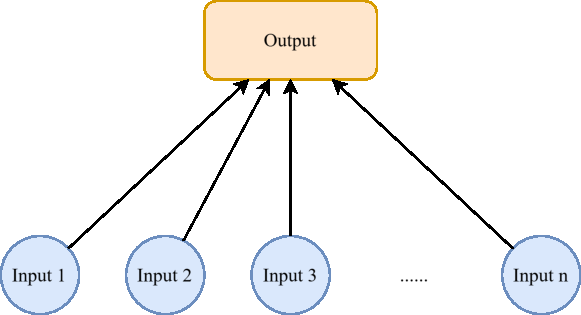
\includegraphics[width = 0.5\textwidth]{chapters/pics/insert_1_linear.pdf}
    \caption{Neural Network Perspective of Linear Regression}
\end{figure}

We can see that the linear regression model is equivalent to a neural network with a single neuron, where the weights and bias correspond to the parameters of the linear model. The loss function remains the same, as we still aim to minimize the Mean Squared Error (MSE) between the predicted outputs and the actual outputs.

For the neural network of linear regression, all the inputs are directly connected to the output neuron without any hidden layers. The output neuron performs a weighted sum of the inputs, adds a bias term, and produces the final output. We call this type of neural network a \textbf{fully-connected layer} or \textbf{dense layer}.

\subsubsection{Some Biology}

In biological neural networks, neurons are interconnected cells that transmit information through electrical and chemical signals. Each neuron consists of a cell body (soma), dendrites (input branches), and an axon (output branch). Dendrites receive signals from other neurons, which are then processed in the cell body. If the signal is strong enough, the neuron generates an action potential (electrical impulse) that travels down the axon to communicate with other neurons.

But nowadays, artificial neural networks are only loosely inspired by biological neural networks. While they share some similarities in terms of structure and function, artificial neural networks are simplified mathematical models that do not capture the full complexity of biological neurons, just like the Russell and Norvig said in their book \textit{Artificial Intelligence: A Modern Approach}.

What we have shown above is just a simple example of how linear regression can be viewed from a neural network perspective. As we delve deeper into the field of machine learning and neural networks, we will explore more complex architectures and techniques that build upon this foundational understanding.

\section{How to Achieve Linear Regression in Practice}

After we know the key idea of linear regression, we can implement it in practice using popular machine learning libraries \textbf{PyTorch}.

Here is a simple example of how to implement linear regression using PyTorch:

\begin{pythoncode}{Libraries}
import random
import torch
\end{pythoncode}

To make things simpler, we will generate some synthetic data for training the linear regression model.

\begin{pythoncode}{Data Generation}
# Generate synthetic data
def generate_data(w, b, num_examples):
    X = torch.normal(0, 1, (num_examples, len(w)))
    y = torch.matmul(X, w) + b
    y += torch.normal(0, 0.01, y.shape)
    return X, y.reshape((-1, 1))

true_w = torch.tensor([2.0, -3.4])
true_b = 4.2
features, labels = generate_data(true_w, true_b, 1000)
\end{pythoncode}

Now we can define the linear regression model using PyTorch's built-in modules. Have a review, we need to read the data, randomly select minibatches, define the model, define the loss function, and optimize the model parameters using Gradient Descent. Now we need to implement these steps in code.

\begin{pythoncode}{Random Minibatch Sampling}
# Define a function to get minibatches
def data_iter(batch_size, features, labels):
    num_examples = len(features)
    indices = list(range(num_examples))
    random.shuffle(indices)
    for i in range(0, num_examples, batch_size):
        batch_indices = torch.tensor(
            indices[i: min(i + batch_size, num_examples)])
        yield features[batch_indices], labels[batch_indices]
\end{pythoncode}

Why we use minibatches? Because using the entire dataset to compute the gradients can be computationally expensive, especially for large datasets. Minibatch SGD allows us to update the model parameters more frequently. Also, take advantage of the \textbf{GPU} acceleration, which can significantly speed up the training process.

Now let's define the linear regression model, first we need to initialize the model parameters (weights and bias):
\begin{pythoncode}{Model Definition}
w = torch.normal(0, 0.01, size=(2, 1), requires_grad=True)
b = torch.zeros(1, requires_grad=True)
\end{pythoncode}

Our next step is to construct the model's forward pass, which computes the predicted outputs given the input features, as well as defining the loss function and the optimization algorithm.

\begin{pythoncode}{Main Components}
# Define the linear regression model
def linreg(X, w, b):
    return torch.matmul(X, w) + b

# Define the Mean Squared Error loss function
def mse_loss(y_hat, y):
    return ((y_hat - y.reshape(y_hat.shape)) ** 2) / 2

# Define the SGD optimization algorithm
def sgd(params, lr, batch_size):
    with torch.no_grad():
        for param in params:
            param -= lr * param.grad / batch_size
            param.grad.zero_()
\end{pythoncode}

Now we can train the linear regression model using the defined components. We will iterate over the training data for a specified number of epochs, updating the model parameters using minibatch SGD.

\begin{pythoncode}{Training Loop}
# Training loop
lr = 0.03
num_epochs = 3
net = linreg
loss = mse_loss

# Main loop
for epoch in range(num_epochs):
    for X, y in data_iter(10, features, labels):
        l = loss(net(X, w, b), y)
        l.sum().backward()
        sgd([w, b], lr, batch_size=10)
    with torch.no_grad():
        train_l = loss(net(features, w, b), labels)
        print(f'epoch {epoch + 1}, loss {float(train_l.mean()):f}')
\end{pythoncode}

In the process of \texttt{l.sum().backward()}, PyTorch automatically computes the gradients of the loss with respect to the model parameters \(w\) and \(b\) using backpropagation. This is one of the key features of PyTorch that simplifies the implementation of machine learning algorithms.

After training the model, we can evaluate its performance by comparing the learned parameters \(w\) and \(b\) with the true parameters used to generate the synthetic data.

\begin{pythoncode}{Model Evaluation}
print(f'Learned weights: {w.reshape(true_w.shape)}')
print(f'Learned bias: {b}')
\end{pythoncode}

To summarize, we have implemented a linear regression model using PyTorch, demonstrating the key steps involved in training the model using minibatch stochastic gradient descent.

We can summarize it step by step as follows:
\begin{enumerate}
    \item Input the training data (features \(X\) and labels \(y\)).
    \item Forward pass: Compute the predicted outputs \(\hat{y}\) using the current model parameters \(w\) and \(b\).
    \item Loss computation: Calculate the loss \(L\) using the Mean Squared Error (MSE) loss function.
    \item Backward pass: Compute the gradients of the loss with respect to the model parameters \(w\) and \(b\) using backpropagation.
    \item Parameter update: Update the model parameters \(w\) and \(b\) using the computed gradients and the learning rate \(\alpha\) with the SGD optimization algorithm.
    \item Repeat steps 2-5 for a predefined number of epochs or until convergence.
\end{enumerate}

You can run the complete code in a Python enviroment with PyTorch installed to see the results. We provide the complete code in the folder for your convenience.

\section{How to Make Things Simpler}

We will introduce some predefined modules in PyTorch that can help us simplify the implementation of linear regression.

Just like what we have done before, we still need to define the model, loss function, and optimization algorithm. But this time, we can use PyTorch's built-in modules to simplify these steps.

Firstly, we still need to generate the synthetic data as before.

\begin{pythoncode}{Data Generation}
import random
import torch
from torch import nn

true_w = torch.tensor([2.0, -3.4])
true_b = 4.2
def generate_data(w, b, num_examples):
    X = torch.normal(0, 1, (num_examples, len(w)))
    y = torch.matmul(X, w) + b
    y += torch.normal(0, 0.01, y.shape)
    return X, y.reshape((-1, 1))

features, labels = generate_data(true_w, true_b, 1000)
\end{pythoncode}

Then, how can we read the data in minibatches? We can use PyTorch's built-in \texttt{DataLoader} module to handle the batching and shuffling of the data for us.

\begin{pythoncode}{DataLoader}
def load_array(data_arrays, batch_size, is_train=True):
    dataset = data.TensorDataset(*data_arrays)
    return data.DataLoader(dataset, batch_size, shuffle=is_train)

batch_size = 10
data_iter = load_array((features, labels), batch_size)
\end{pythoncode}

Next, we can define the linear regression model using PyTorch's \texttt{nn.Linear} module, which automatically handles the initialization of weights and biases for us.

\begin{pythoncode}{Model Definition}
# Define the linear regression model using nn.Linear
net = nn.Linear(2, 1)
\end{pythoncode}

Next, we can define the loss function using PyTorch's built-in \texttt{nn.MSELoss} module, which implements the Mean Squared Error loss function.
\begin{pythoncode}{Loss Function}
# Define the Mean Squared Error loss function using nn.MSELoss
loss = nn.MSELoss()
\end{pythoncode}

Finally, we can define the optimization algorithm using PyTorch's \texttt{torch.optim.SGD} module, which implements the Stochastic Gradient Descent optimization algorithm.
\begin{pythoncode}{Optimizer}
# Define the SGD optimization algorithm using torch.optim.SGD
trainer = torch.optim.SGD(net.parameters(), lr=0.03)
\end{pythoncode}

Now we can train the linear regression model using the defined components. The training loop remains similar to the previous implementation, but we can leverage the built-in modules to simplify the code.
\begin{pythoncode}{Training Loop}
# Training loop
num_epochs = 3
for epoch in range(num_epochs):
    for X, y in data_iter:
        l = loss(net(X), y)
        trainer.zero_grad()
        l.backward()
        trainer.step()
    l = loss(net(features), labels)
    print(f'epoch {epoch + 1}, loss {l:f}')
\end{pythoncode}

After training the model, we can evaluate its performance by comparing the learned parameters with the true parameters used to generate the synthetic data.

\begin{pythoncode}{Model Evaluation}
w = net.weight.data
b = net.bias.data
\end{pythoncode}

\section{Softmax Regression}

Softmax regression, also known as multinomial logistic regression, is an extension of linear regression that is used for multi-class classification problems. Unlike linear regression, which predicts continuous output values, softmax regression predicts the probabilities of each class for a given input.

\subsection{Model Definition}

The output of the softmax regression model is a probability distribution of each class. Considering a picture classification task with \(k\) classes, the output of the model is a \(k\)-dimensional vector, where each element represents the predicted probability of the input belonging to that class. The sum of all probabilities in the output vector is equal to 1.

So here comes the first question, how to choose the labels for multi-class classification? The answer is to use \textbf{one-hot encoding}.

\begin{definition}

One-hot encoding is a technique used to represent categorical variables as binary vectors. In one-hot encoding, each category is represented by a vector of length equal to the number of categories, where all elements are 0 except for the element corresponding to the category, which is set to 1.
\end{definition}

After defining the labels, we can define the softmax regression model. The model can be expressed as follows:
\[
o_1 = x_1 w_{11} + x_2 w_{12} + x_3 w_{13} + x_4 w_{14} + b_1
\]
\[
o_2 = x_1 w_{21} + x_2 w_{22} + x_3 w_{23} + x_4 w_{24} + b_2
\]
\[
o_3 = x_1 w_{31} + x_2 w_{32} + x_3 w_{33} + x_4 w_{34} + b_3
\]

where \(o_i\) is the output score for class \(i\), \(x_j\) is the input feature \(j\), \(w_{ij}\) is the weight connecting input feature \(j\) to class \(i\), and \(b_i\) is the bias term for class \(i\).

We can use a picture to illustrate the model structure:
\begin{figure}[h]
    \centering
    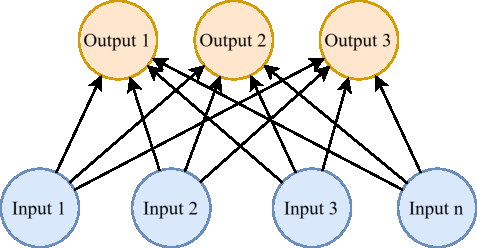
\includegraphics[width = 0.5\textwidth]{chapters/pics/insert_2_softmax.pdf}
    \caption{Softmax Regression Model Structure}
\end{figure}

\newpage

Now we have the output scores for each class, but we need to convert these scores into probabilities. This is where the softmax function comes into play.

We cannot directly use the output scores for classification, as they can be any real number and do not represent probabilities. The softmax function transforms the output scores into probabilities by applying the following formula:

\[
P(y = i | x) = \frac{e^{o_i}}{\sum_{j=1}^{k} e^{o_j}}
\]

where \(P(y = i | x)\) is the predicted probability of class \(i\) given input \(x\), \(o_i\) is the output score for class \(i\), and \(k\) is the total number of classes.

Althougn the softmax function is not linear, the model is still called softmax regression because the output scores \(o_i\) are computed using a linear combination of the input features. Thus, softmax regression can be seen as a linear model followed by a non-linear activation function (softmax) to produce probabilities.

We also need to define the loss function for softmax regression. The most commonly used loss function for multi-class classification is the Cross-Entropy Loss, which measures the difference between the predicted probability distribution and the true distribution (one-hot encoded labels).

The Cross-Entropy Loss can be expressed as follows:
\[
L = -\sum_{i=1}^{k} y_i \ln(P(y = i | x))
\]

We can derive the loss function from the likelihood function, just like what we have done in linear regression. Given a training dataset with \(m\) examples, the likelihood function for the entire dataset can be expressed as the product of the individual likelihoods for each training example:
\[
L(w, b) = \prod_{i=1}^{m} P(y^{(i)} | x^{(i)}; w, b)
\]
Taking the natural logarithm of the likelihood function, we have:
\[
\ln L(w, b) = \sum_{i=1}^{m} \ln(P(y^{(i)} | x^{(i)}; w, b))
\]
Maximizing the log-likelihood function is equivalent to minimizing the negative log-likelihood. Ignoring the constant terms, we can focus on minimizing the following expression:
\[
-\sum_{i=1}^{m} \sum_{j=1}^{k} y_j^{(i)} \ln(P(y = j | x^{(i)}; w, b))
\]
This is exactly the Cross-Entropy Loss function we defined earlier for softmax regression. Therefore, by maximizing the likelihood of the observed data given the model parameters, we arrive at the conclusion that minimizing the Cross-Entropy Loss function is equivalent to maximizing the likelihood.

For how to derive the Cross-Entropy Loss function in detail, please refer to the content about \textbf{Information Theory} on the internet.

\newpage

\subsection{MNIST}

The MNIST dataset is a widely used benchmark dataset for image classification tasks, particularly for handwritten digit recognition. It consists of 60,000 training images and 10,000 test images of handwritten digits (0-9), each represented as a 28x28 grayscale image.

In this section, we will implement softmax regression using PyTorch to classify the Fashion-MNIST dataset. We will follow similar steps as in the previous linear regression example, but with modifications to accommodate the multi-class classification task.

\begin{pythoncode}{Libraries}
import torch
import torchvision
from torch.utils import data
from torchvision import transforms
\end{pythoncode}

Now we will load the Fashion-MNIST dataset using PyTorch's \texttt{torchvision} module. We will apply necessary transformations to the images, such as converting them to tensors and normalizing the pixel values.

\begin{pythoncode}{Data Loading}
# Load the Fashion-MNIST dataset
trans = transforms.ToTensor()
mnist_train = torchvision.datasets.FashionMNIST(
    root="../data", train=True, transform=trans, download=True)
mnist_test = torchvision.datasets.FashionMNIST(
    root="../data", train=False, transform=trans, download=True)
\end{pythoncode}

As we have already known, the \textbf{Fashion-MNIST} dataset contains 10 classes of clothing items, including T-shirts, trousers, pullovers, dresses, coats, sandals, shirts, sneakers, bags, and ankle boots. Each image is a 28x28 grayscale image, which we will flatten into a 784-dimensional vector for input to the softmax regression model.

Now let's define the data loader to read the data in minibatches.

\begin{pythoncode}{DataLoader}
batch_size = 256
train_iter = data.DataLoader(mnist_train, batch_size, shuffle=True, num_workers=4)
\end{pythoncode}

Now we can define the function \texttt{load\_data\_fashion\_mnist} to encapsulate the data loading process for convenience.

\begin{pythoncode}{Data Loading Function}
def load_data_fashion_mnist(batch_size, resize=None):
    trans = [transforms.ToTensor()]
    if resize:
        trans.insert(0, transforms.Resize(resize))
    trans = transforms.Compose(trans)
    mnist_train = torchvision.datasets.FashionMNIST(
        root="../data", train=True, transform=trans, download=True)
    mnist_test = torchvision.datasets.FashionMNIST(
        root="../data", train=False, transform=trans, download=True)
    return (data.DataLoader(mnist_train, batch_size, shuffle=True,
                            num_workers=get_dataloader_workers()),
            data.DataLoader(mnist_test, batch_size, shuffle=False,
                            num_workers=get_dataloader_workers()))
\end{pythoncode}

The parameter "resize" allows us to resize the images if needed. The function returns the training and test data loaders.

Now we can define the softmax regression model using PyTorch's \texttt{nn.Linear} module, which automatically handles the initialization of weights and biases for us.

Firstly let's initialize the model parameters (weights and bias):

\begin{pythoncode}{Model Definition}
num_inputs = 784
num_outputs = 10

W = torch.normal(0, 0.01, size=(num_inputs, num_outputs), requires_grad=True)
b = torch.zeros(num_outputs, requires_grad=True)
\end{pythoncode}

Then we can define the softmax regression model, loss function, and optimization algorithm.

\begin{pythoncode}{Main Components}
# Define the softmax regression model
def softmax(X):
    X_exp = torch.exp(X)
    partition = X_exp.sum(1, keepdim=True)
    return X_exp / partition
\end{pythoncode}

During the process of calculating the softmax function, we use the \texttt{keepdim=True} parameter to ensure that the output tensor maintains the same number of dimensions as the input tensor. This is important for subsequent operations, such as loss calculation, where we need to align the dimensions of the predicted probabilities and the true labels. Also, we use the \textbf{broadcasting} feature of PyTorch to perform element-wise division between the exponentiated scores and the partition function.

\begin{pythoncode}{Loss Function and Optimizer}
# Define the cross-entropy loss function
def net(X):
    return softmax(torch.matmul(X.reshape((-1, W.shape[0])), W) + b)

# Define the cross-entropy loss function
def cross_entropy(y_hat, y):
    return -torch.log(y_hat[range(len(y_hat)), y])
\end{pythoncode}

Instead of computing the loss using the full formula that sums over all classes, this implementation uses an efficient indexing trick. The expression \texttt{y\_hat[range(len(y\_hat)), y]} performs advanced indexing:

\begin{enumerate}
    \item For each sample in the batch, it selects the predicted probability corresponding to the true class label \(y\).
    \item This results in a 1-dimensional tensor containing the predicted probabilities for the correct classes for all samples in the batch.
    \item Finally, the negative logarithm of these probabilities is computed to obtain the cross-entropy loss for each sample.
\end{enumerate}

It is logically equivalent to the function below:

\begin{pythoncode}

def cross_entropy_onehot(y_hat, y):
    y_onehot = torch.zeros_like(y_hat)
    y_onehot[range(len(y_hat)), y] = 1
    return -(y_onehot * torch.log(y_hat)).sum(dim=1)
\end{pythoncode}

But the first implementation is more efficient in terms of computation and memory usage.

Afterall, we have defined the loss function. However, in real life applications, we need to output the predicted class labels based on the predicted probabilities. This can be achieved using the \texttt{argmax} function, which returns the index of the maximum value along a specified dimension.

\begin{pythoncode}{Prediction Function}
def accuracy(y_hat, y):
    if len(y_hat.shape) > 1 and y_hat.shape[1] > 1:
        y_hat = y_hat.argmax(axis=1)
    cmp = y_hat.type(y.dtype) == y
    return float(cmp.type(y.dtype).sum())
\end{pythoncode}

Here we define a class \texttt{Accumulator} to help us accumulate the sum of multiple variables over time, which is useful for tracking metrics like loss and accuracy during training.

\begin{pythoncode}{Accumulator Class}
class Accumulator:
    def __init__(self, n):
        self.data = [0.0] * n

    def add(self, *args):
        self.data = [a + float(b) for a, b in zip(self.data, args)]

    def reset(self):
        self.data = [0.0] * len(self.data)

    def __getitem__(self, idx):
        return self.data[idx]
\end{pythoncode}

Finally, we can define the training function to encapsulate the training process for convenience.

\begin{pythoncode}{Training Function}
def train_epoch_ch3(net, train_iter, loss, updater):
    if isinstance(net, torch.nn.Module):
        net.train()
    metric = Accumulator(3)
    for X, y in train_iter:
        y_hat = net(X)
        l = loss(y_hat, y).sum()
        if isinstance(updater, torch.optim.Optimizer):
            updater.zero_grad()
            l.backward()
            updater.step()
        else:
            l.backward()
            updater(X.shape[0])
        metric.add(float(l), accuracy(y_hat, y), y.numel())
    return metric[0] / metric[2], metric[1] / metric[2]
\end{pythoncode}

The training function defined above trains the model for only one epoch. To evaluate the model's performance on the test dataset, we need a function to compute the accuracy on the test set.

\begin{pythoncode}{Evaluation Function}
def evaluate_accuracy(net, data_iter):
    if isinstance(net, torch.nn.Module):
        net.eval()
    metric = Accumulator(2)
    with torch.no_grad():
        for X, y in data_iter:
            metric.add(accuracy(net(X), y), y.numel())
    return metric[0] / metric[1]
\end{pythoncode}

Now we can combine everything to define the complete training loop, which iterates through multiple epochs, trains the model, and evaluates its performance on the test dataset at the end of each epoch.

\begin{pythoncode}{Complete Training Loop}
def train_ch3(net, train_iter, test_iter, loss, num_epochs, updater):
    for epoch in range(num_epochs):
        train_metrics = train_epoch_ch3(net, train_iter, loss, updater)
        test_acc = evaluate_accuracy(net, test_iter)
        print(f'epoch {epoch + 1}, loss {train_metrics[0]:.4f}, '
              f'train acc {train_metrics[1]:.3f}, test acc {test_acc:.3f}')
\end{pythoncode}

With all the components in place, we can now train the model.

\begin{pythoncode}{Run Training}
num_epochs = 10
lr = 0.1

def updater(batch_size):
    return torch.optim.SGD([W, b], lr=lr)

train_ch3(net, train_iter, mnist_test, cross_entropy, num_epochs, updater)
\end{pythoncode}

Before making predictions, we need to define some helper functions to visualize the images and labels. We also need to import \texttt{matplotlib.pyplot}.

\begin{pythoncode}{Visualization Helpers}
import matplotlib.pyplot as plt

def get_fashion_mnist_labels(labels):
    text_labels = ['t-shirt', 'trouser', 'pullover', 'dress', 'coat',
                   'sandal', 'shirt', 'sneaker', 'bag', 'ankle boot']
    return [text_labels[int(i)] for i in labels]

def show_images(imgs, num_rows, num_cols, titles=None, scale=1.5):
    figsize = (num_cols * scale, num_rows * scale)
    _, axes = plt.subplots(num_rows, num_cols, figsize=figsize)
    axes = axes.flatten()
    for i, (ax, img) in enumerate(zip(axes, imgs)):
        if torch.is_tensor(img):
            ax.imshow(img.numpy())
        else:
            ax.imshow(img)
        ax.axes.get_xaxis().set_visible(False)
        ax.axes.get_yaxis().set_visible(False)
        if titles:
            ax.set_title(titles[i])
    return axes
\end{pythoncode}

After training, we can use the trained model to make predictions on some images from the test dataset.

\begin{pythoncode}{Prediction}
def predict_ch3(net, test_iter, n=6):
    for X, y in test_iter:
        break
    trues = get_fashion_mnist_labels(y)
    preds = get_fashion_mnist_labels(net(X).argmax(axis=1))
    titles = [true +'\n' + pred for true, pred in zip(trues, preds)]
    show_images(X[0:n].reshape((n, 28, 28)), 1, n, titles=titles[0:n])

predict_ch3(net, mnist_test)
\end{pythoncode}

This concludes the implementation of Softmax Regression using PyTorch. The model is now capable of classifying images from the Fashion-MNIST dataset with reasonable accuracy.

You can run the complete code in a Python enviroment with PyTorch and torchvision installed to see the results. We provide the complete code in the folder for your convenience.

Now you have learned how to implement both Linear Regression and Softmax Regression using PyTorch. These foundational techniques are essential for understanding more complex machine learning models and algorithms that will be covered in later chapters.

In the next chapter, we will explore a real neural network architecture called \textbf{Multilayer Perceptron (MLP)}, which builds upon the concepts learned in this chapter and introduces additional layers and non-linear activation functions to enhance the model's capacity to learn complex patterns in data.

\chapter{Multilayer Perceptrons}

In this chapter, we will explore the first type of neural network architecture: the multilayer perceptron (MLP). MLPs are a class of feedforward artificial neural networks that consist of multiple layers of nodes, or neurons, each fully connected to the next layer. They are widely used for various machine learning tasks, including classification and regression.


\end{document}
